\chapter{Porównanie algorytmów ESRGAN i DWSR} \label{chap:porownanie_algorytmow}

Skoro mamy narzędzie pozwalające korzystać algorytmów \textbf{DWSR} \cite{guo2017deep} i \textbf{ESRGAN} \cite{wang2018esrgan} do zadania super-rozdzielczości, to warto porównać te metody. W tym rozdziale zostanie przeprowadzona analiza porównawcza algorytmów, oceniona zostanie jakość rekonstruowanych obrazów, szybkość działania oraz złożoność implementacji algorytmów.

Do testów algorytmów wykorzystałem zestaw testowy z repozytorium \textbf{DWSR} \cite{guo2017deep}. Wybór padł na ten zestaw, gdyż obrazy te nie były wykorzystywane w treningu żadnej z implementowanych sieci. Obrazy w tym zestawie minimalnie różnią się od siebie rozdzielczością, co pozwala na dokładniejsze porównanie algorytmów zwłaszcza w kontekście analizy wydajności.

\section{Jakość odtwarzania obrazów}

W tym rozdziale przedstawię wyniki testów jakości odtwarzania obrazów przez algorytmy \textbf{DWSR} i \textbf{ESRGAN}.
Dokonałem selekcji obrazów - wybrałem te, które najlepiej obrazują różnice pomiędzy wynikami działania algorytmów.


Na obrazie \ref{fig:image100}. możemy sprawdzić jak algorytmy radzą sobie z rekonstrukcją tekstur drzew i liści. Widać, że algorytm \textbf{DWSR} radzi sobie bardzo dobrze z zachowaniem kierunku tekstur, co zawdzięcza transformacji falkowej, lecz detale nie są odwzorowane idealnie. Algorytm \textbf{ESRGAN} dużo lepiej poradził sobie z odwzorowaniem detali i tekstur. Obrazy odwzorowane przez ten algorytm są bardzo ostre, miejscami aż nienaturalnie. 

\begin{figure}[H]
    \centering
    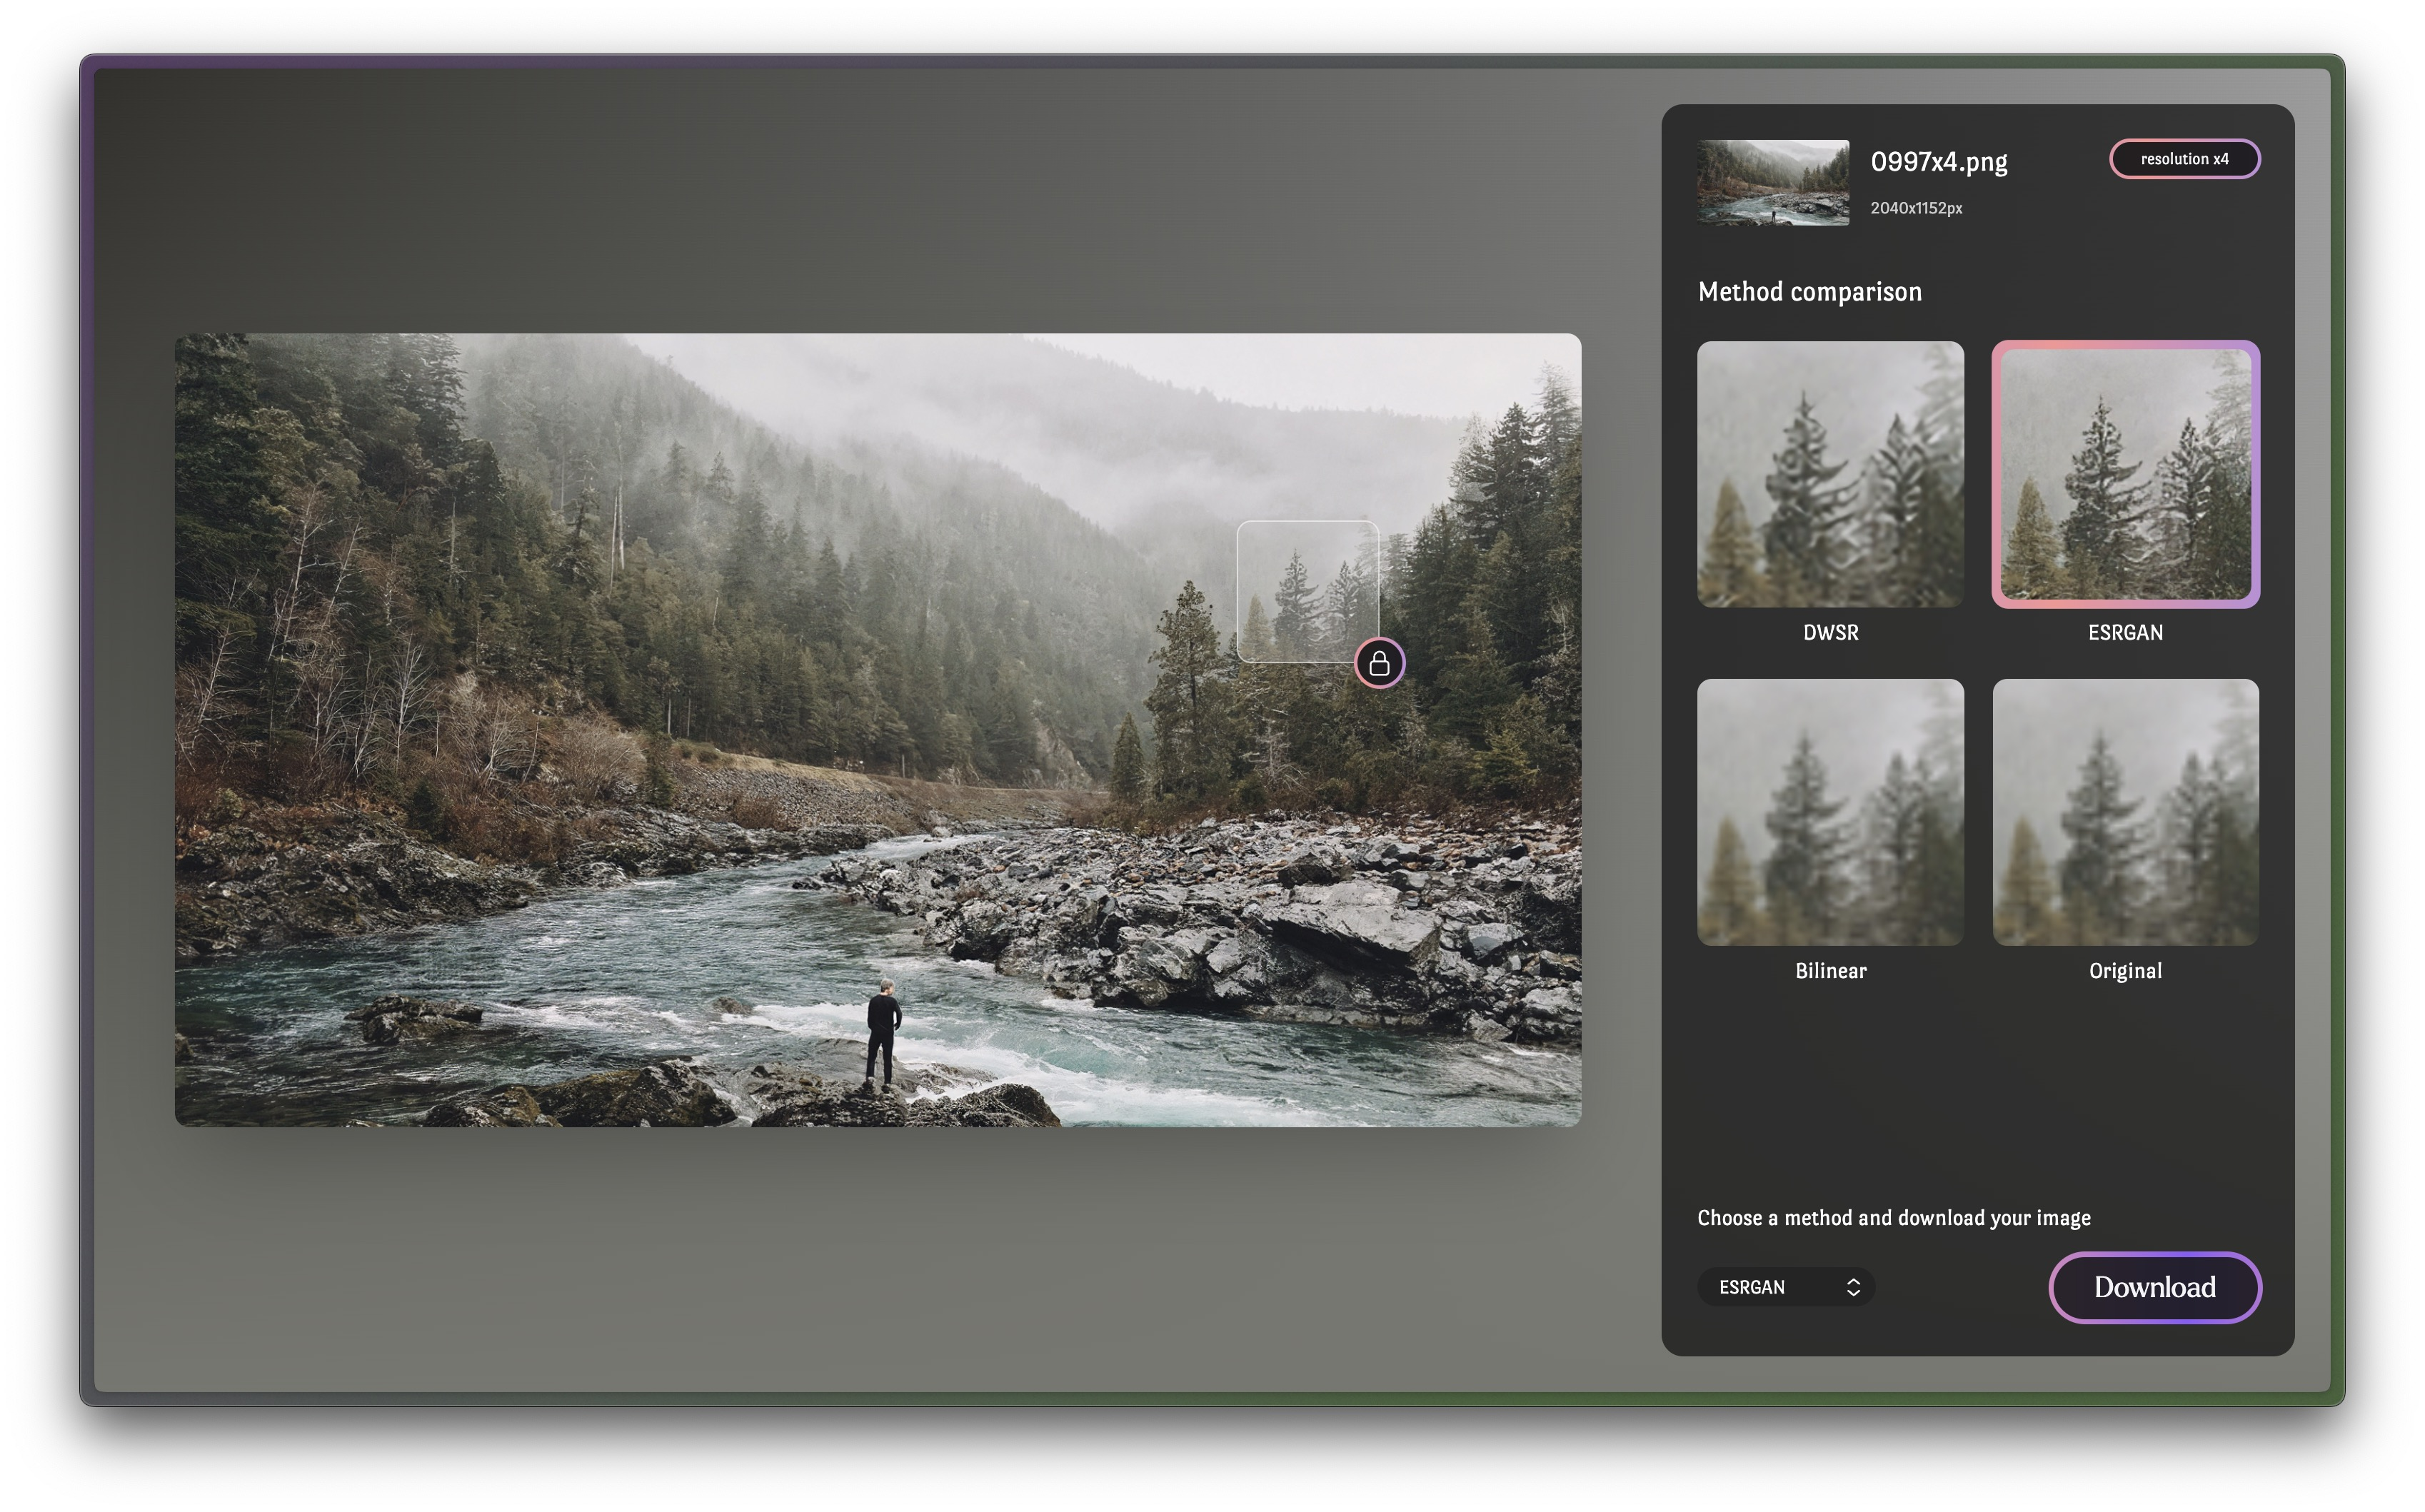
\includegraphics[width=0.9\linewidth]{Rozdziały/05.Porownanie_algorytmow/Obrazy/Zrzut ekranu 2023-12-12 o 14.13.48.jpg}  
    \caption{Obraz \textit{0997x4.png} z zestawu testowego \cite{guo2017deep}}
    \label{fig:image100}
\end{figure}

Na obrazie \ref{fig:image101} możemy sprawdzić jak algorytmy radzą sobie z rekonstrukcją detali twarzy. Na tym przykładzie widać, że algorytm \textbf{ESRGAN} halucynuje detale twarzy i te wyglądają bardzo nienaturalnie, jednak braz wygenerowany przez ten algorytm jest bardzo ostry. Algorytm \textbf{DWSR} radzi sobie dużo lepiej z zachowaniem naturalnego wyglądu twarzy, lecz nie odwzorowuje detali tak dobrze jak \textbf{ESRGAN}.

\begin{figure}[ht]
    \centering
    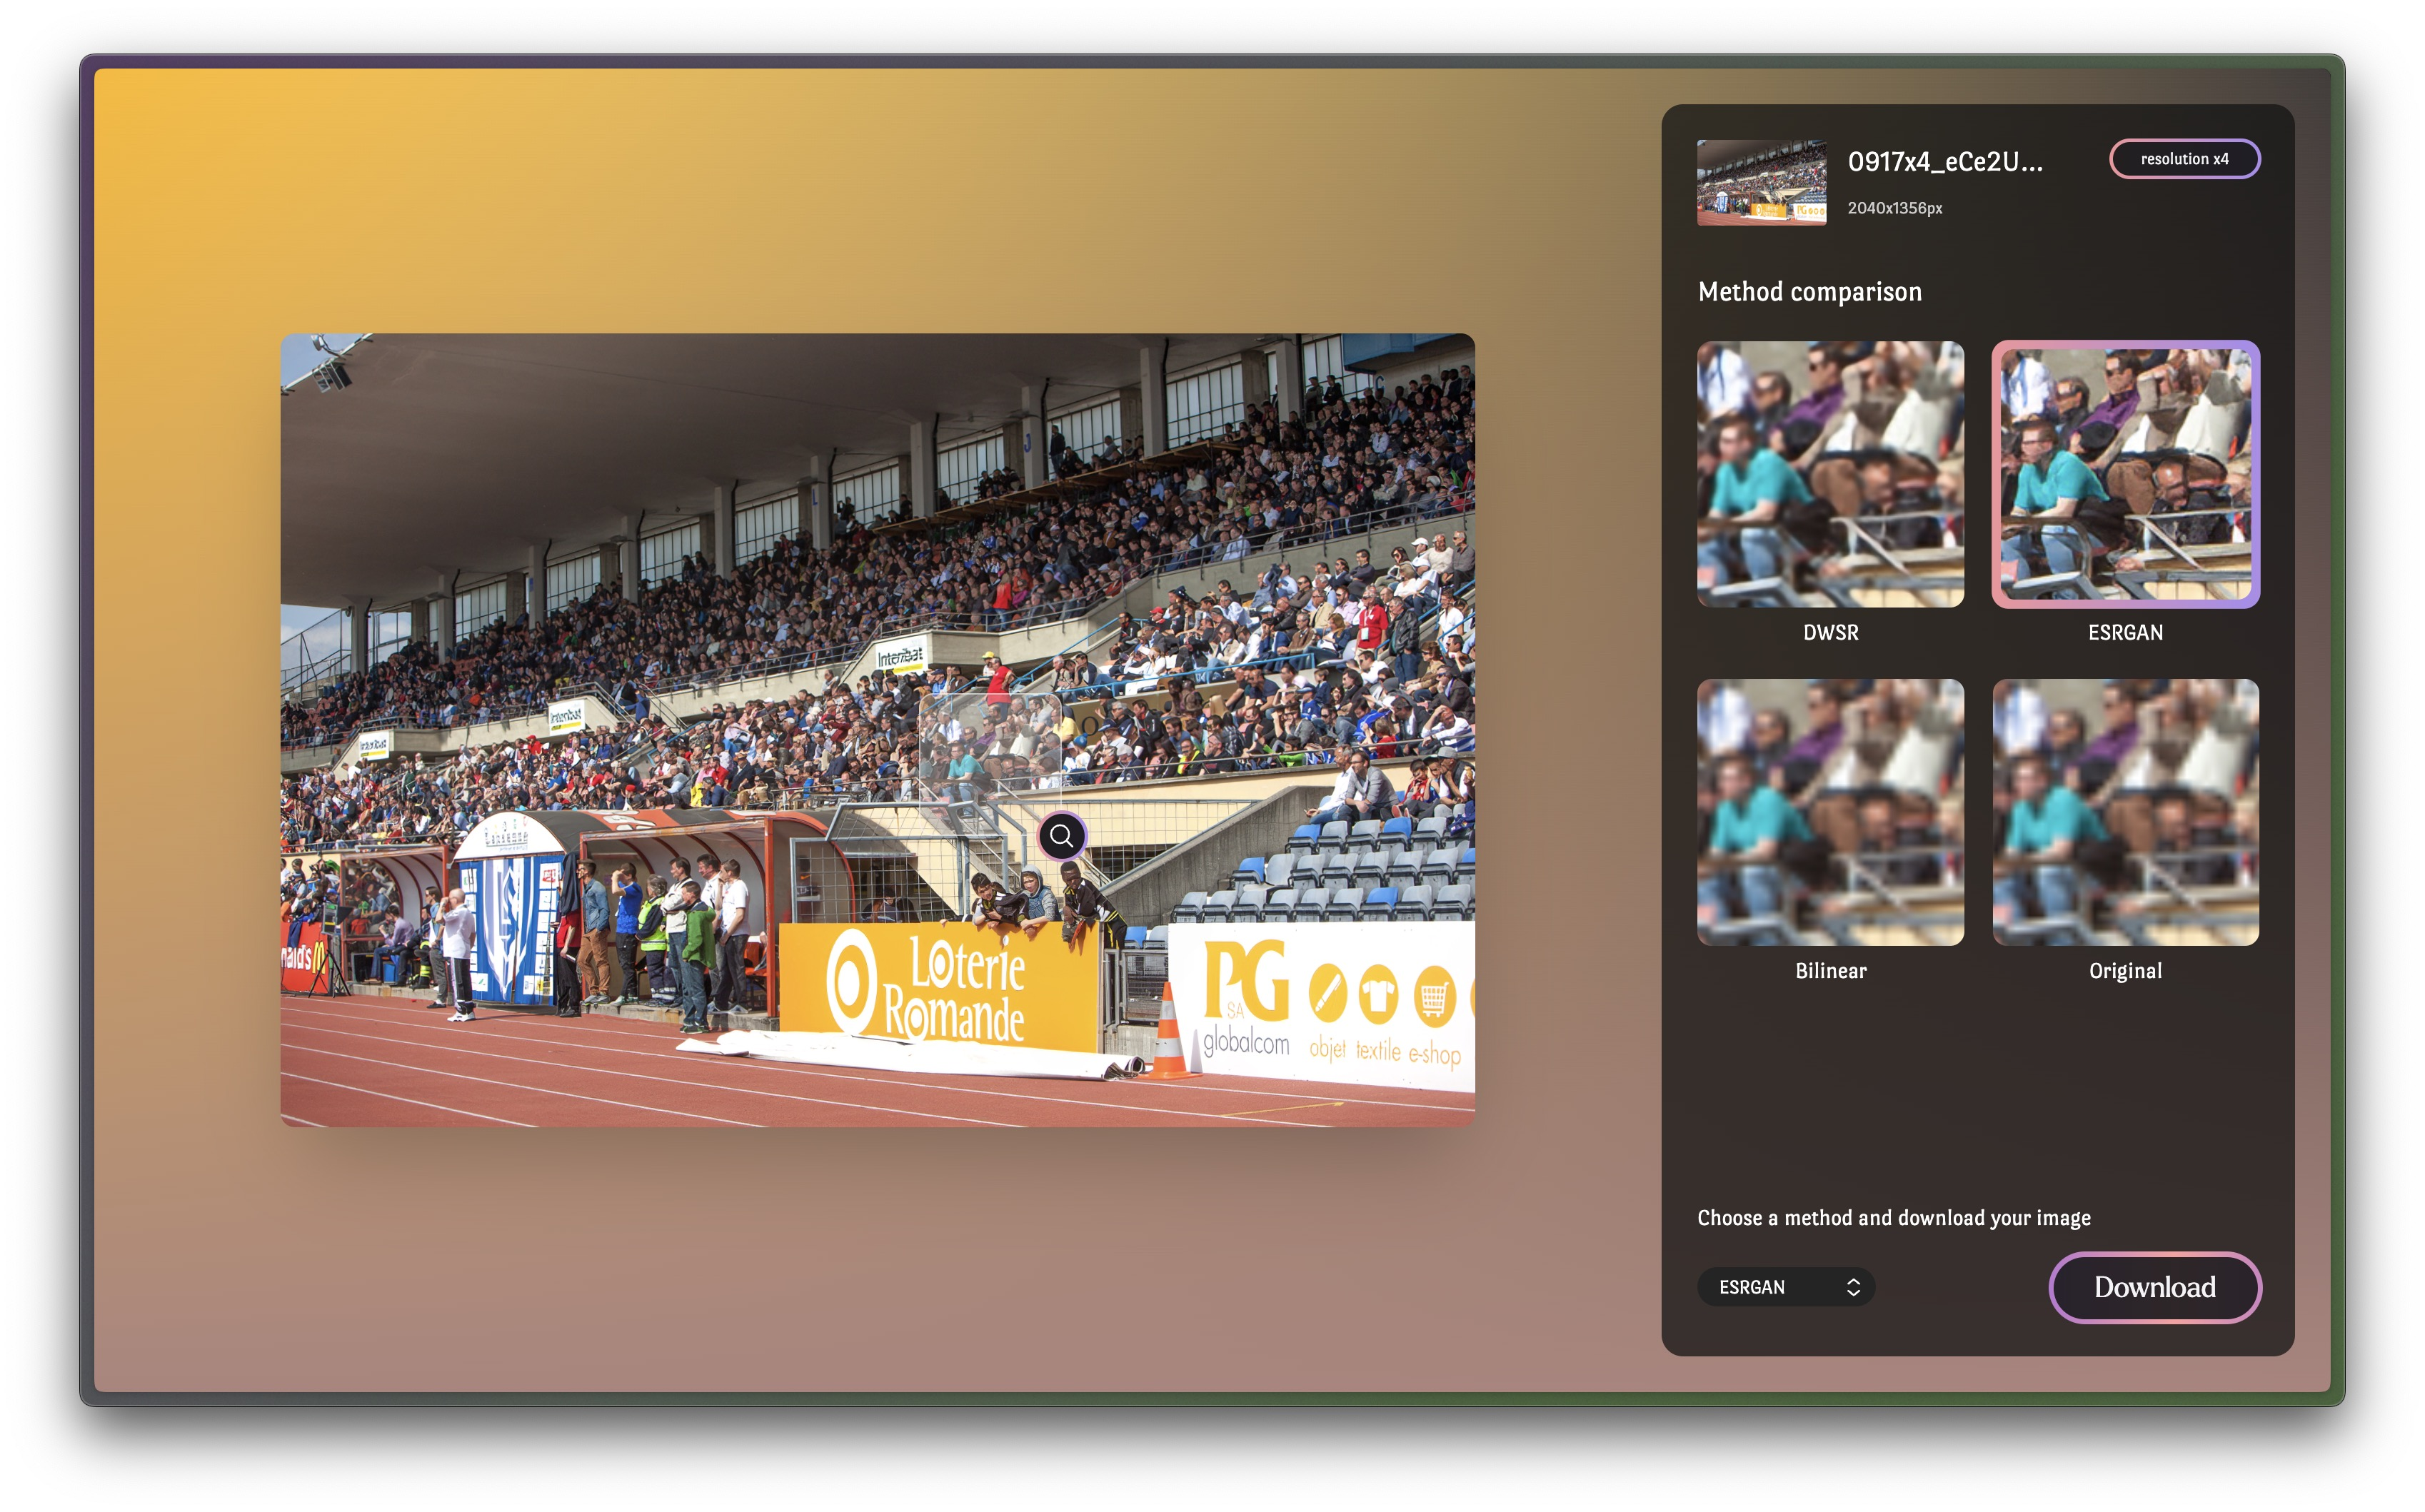
\includegraphics[width=0.9\linewidth]{Rozdziały/05.Porownanie_algorytmow/Obrazy/Zrzut ekranu 2023-12-12 o 14.11.49.jpg}  
    \caption{Obraz \textit{0917x4.png} z zestawu testowego \cite{guo2017deep}}
    \label{fig:image101}
\end{figure}

Na obrazie \ref{fig:image102} możemy się przekonać jak algorytmy radzą sobie z powiększeniem obrazu, na którym zdecydowanie dominują niskie częstotliwości, ale występują też krzywe z ostrzejszymi krawędziami. Tutaj świetnie sprawdził się algorytm \textbf{DWSR}, który zachował naturalny wygląd obrazu, dodatkowo zachowując ostrość krawędzi. Algorytm \textbf{ESRGAN} również poradził sobie bardzo dobrze. Na tego typu obrazach algorytm \textbf{Bilinear} (interpolacja dwuliniowa), również radzi sobie przyzwoicie, ale niestety krawędzie w obrazie wynikowym są bardzo rozmyte.

\begin{figure}[H]
    \centering
    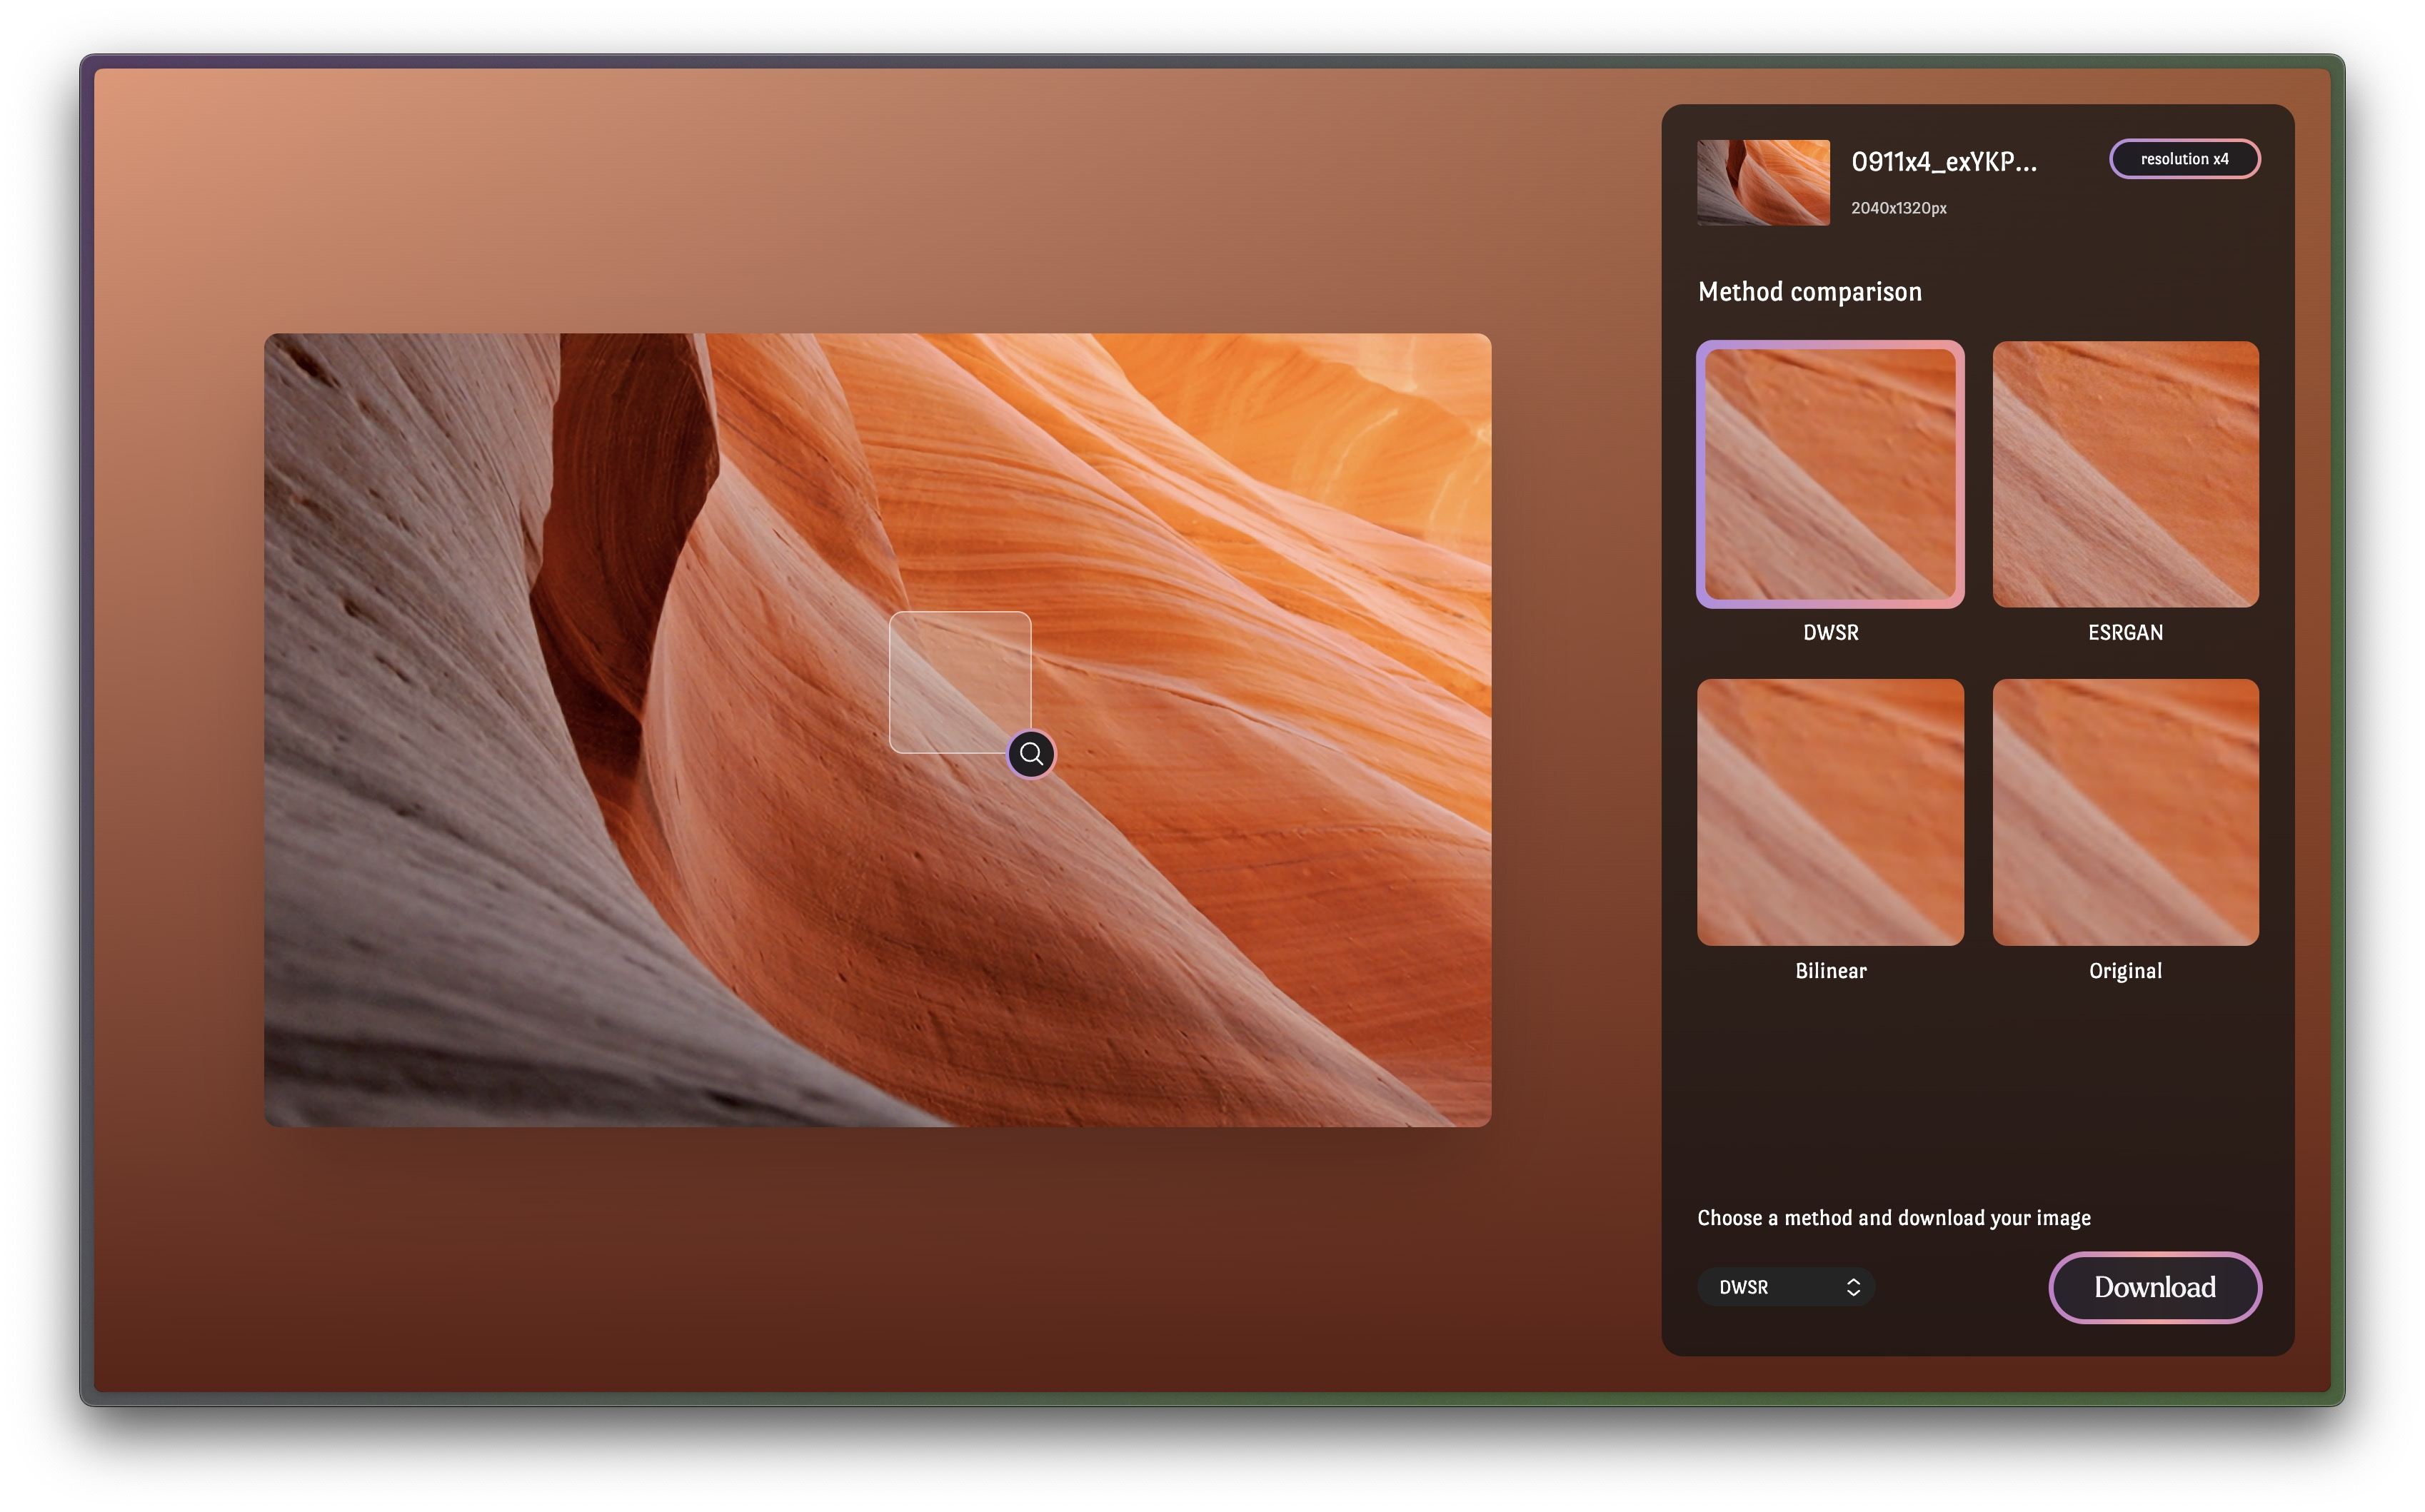
\includegraphics[width=0.9\linewidth]{Rozdziały/05.Porownanie_algorytmow/Obrazy/Zrzut ekranu 2023-12-12 o 14.12.47.jpg}  
    \caption{Obraz \textit{0911x4.png} z zestawu testowego \cite{guo2017deep}}
    \label{fig:image102}
\end{figure}

Obraz testowy \ref{fig:image103} jest bardzo dobrym przykładem scenerii z dużą ilością detali i tekstur. Algorytm \textbf{ESRGAN} bezbłędnie poradził sobie z rekonstrukcją detali takich jak budynki, czy ulice. Algorytm \textbf{DWSR} również poradził sobie dobrze, jednak obraz nie jest nawet bliski ostrości jaką osiągnął algorytm \textbf{ESRGAN}.

\begin{figure}[H]
    \centering
    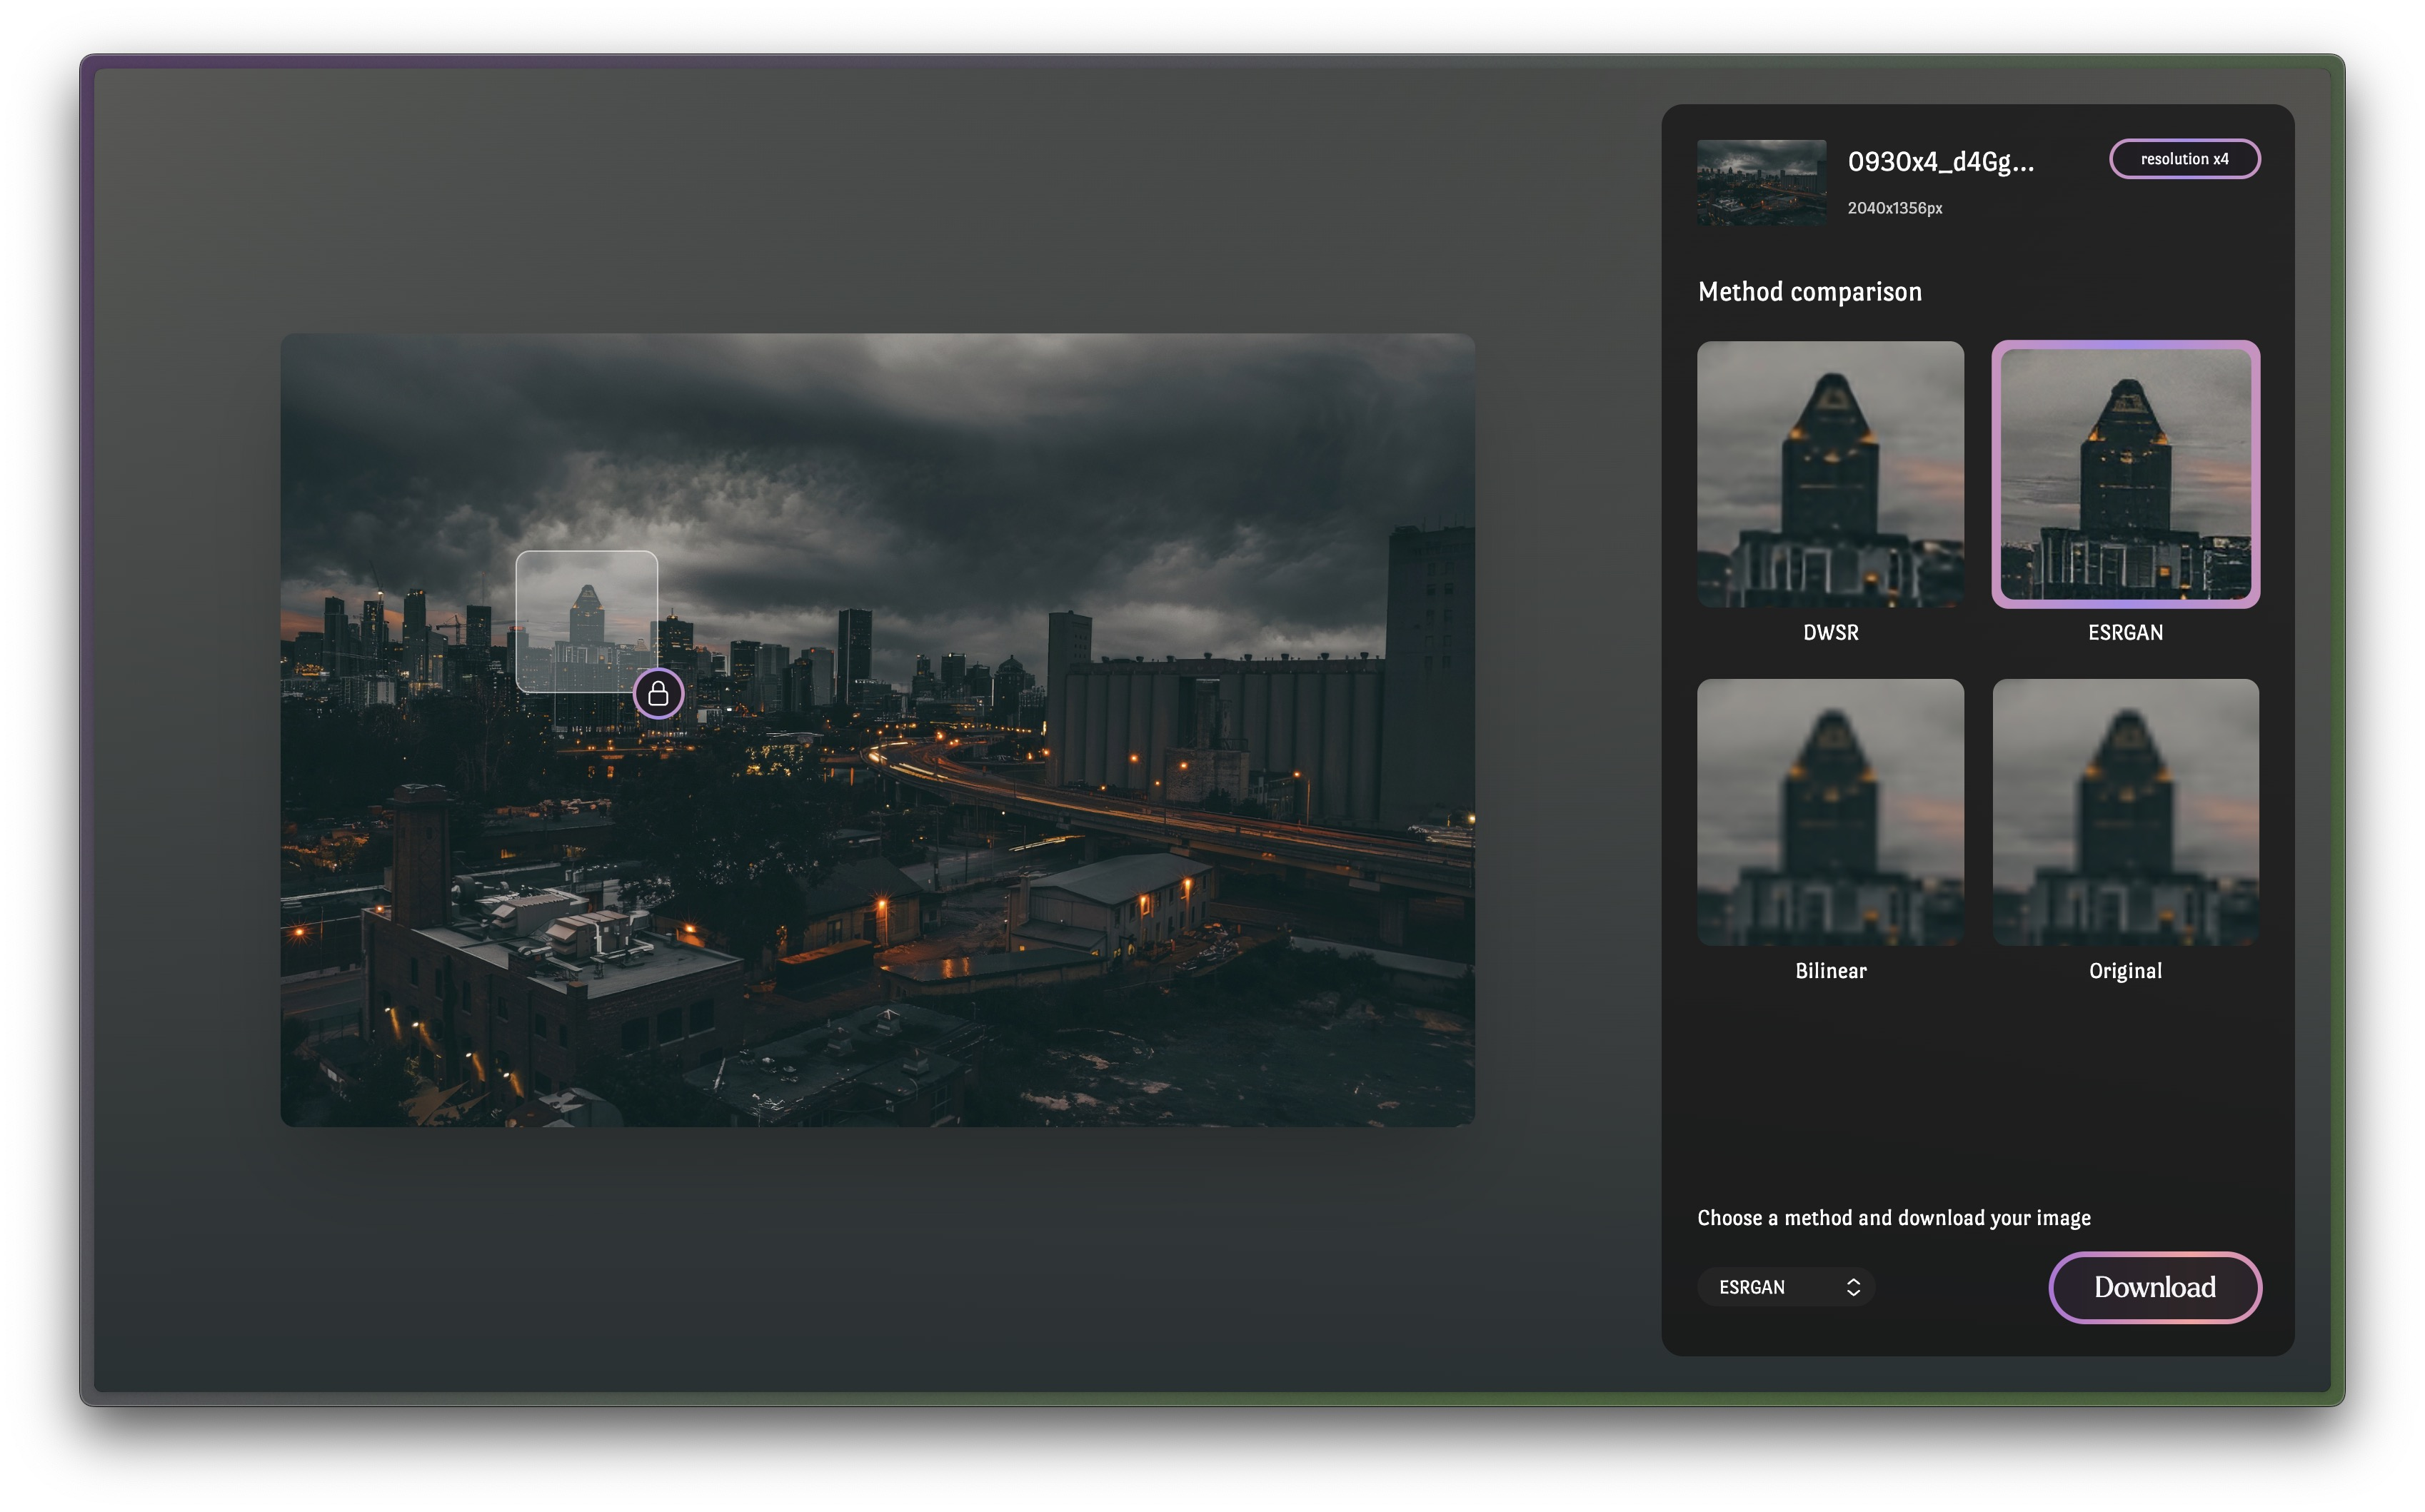
\includegraphics[width=0.9\linewidth]{Rozdziały/05.Porownanie_algorytmow/Obrazy/Zrzut ekranu 2023-12-12 o 14.12.20.jpg}  
    \caption{Obraz \textit{0930x4.png} z zestawu testowego \cite{guo2017deep}}
    \label{fig:image103}
\end{figure}

Obraz testowy \ref{fig:image104} jest przykładem działania algorytmów, gdy mamy do czynienia z obrazem o bardzo niskiej rozdzielczości. Algorytm \textbf{ESRGAN} poradził sobie bardzo dobrze ze stworzeniem detali. Dokładnie zarysowane są wszystkie linie, ale obraz miejscami odbiega od oryginału, widać to między innymi na oku postaci. Algorytm \textbf{DWSR} poradził sobie dobrze, odtworzenie detali jest bliskie oryginałowi ale obraz jest bardzo rozmyty.


\begin{figure}[H]
    \centering
    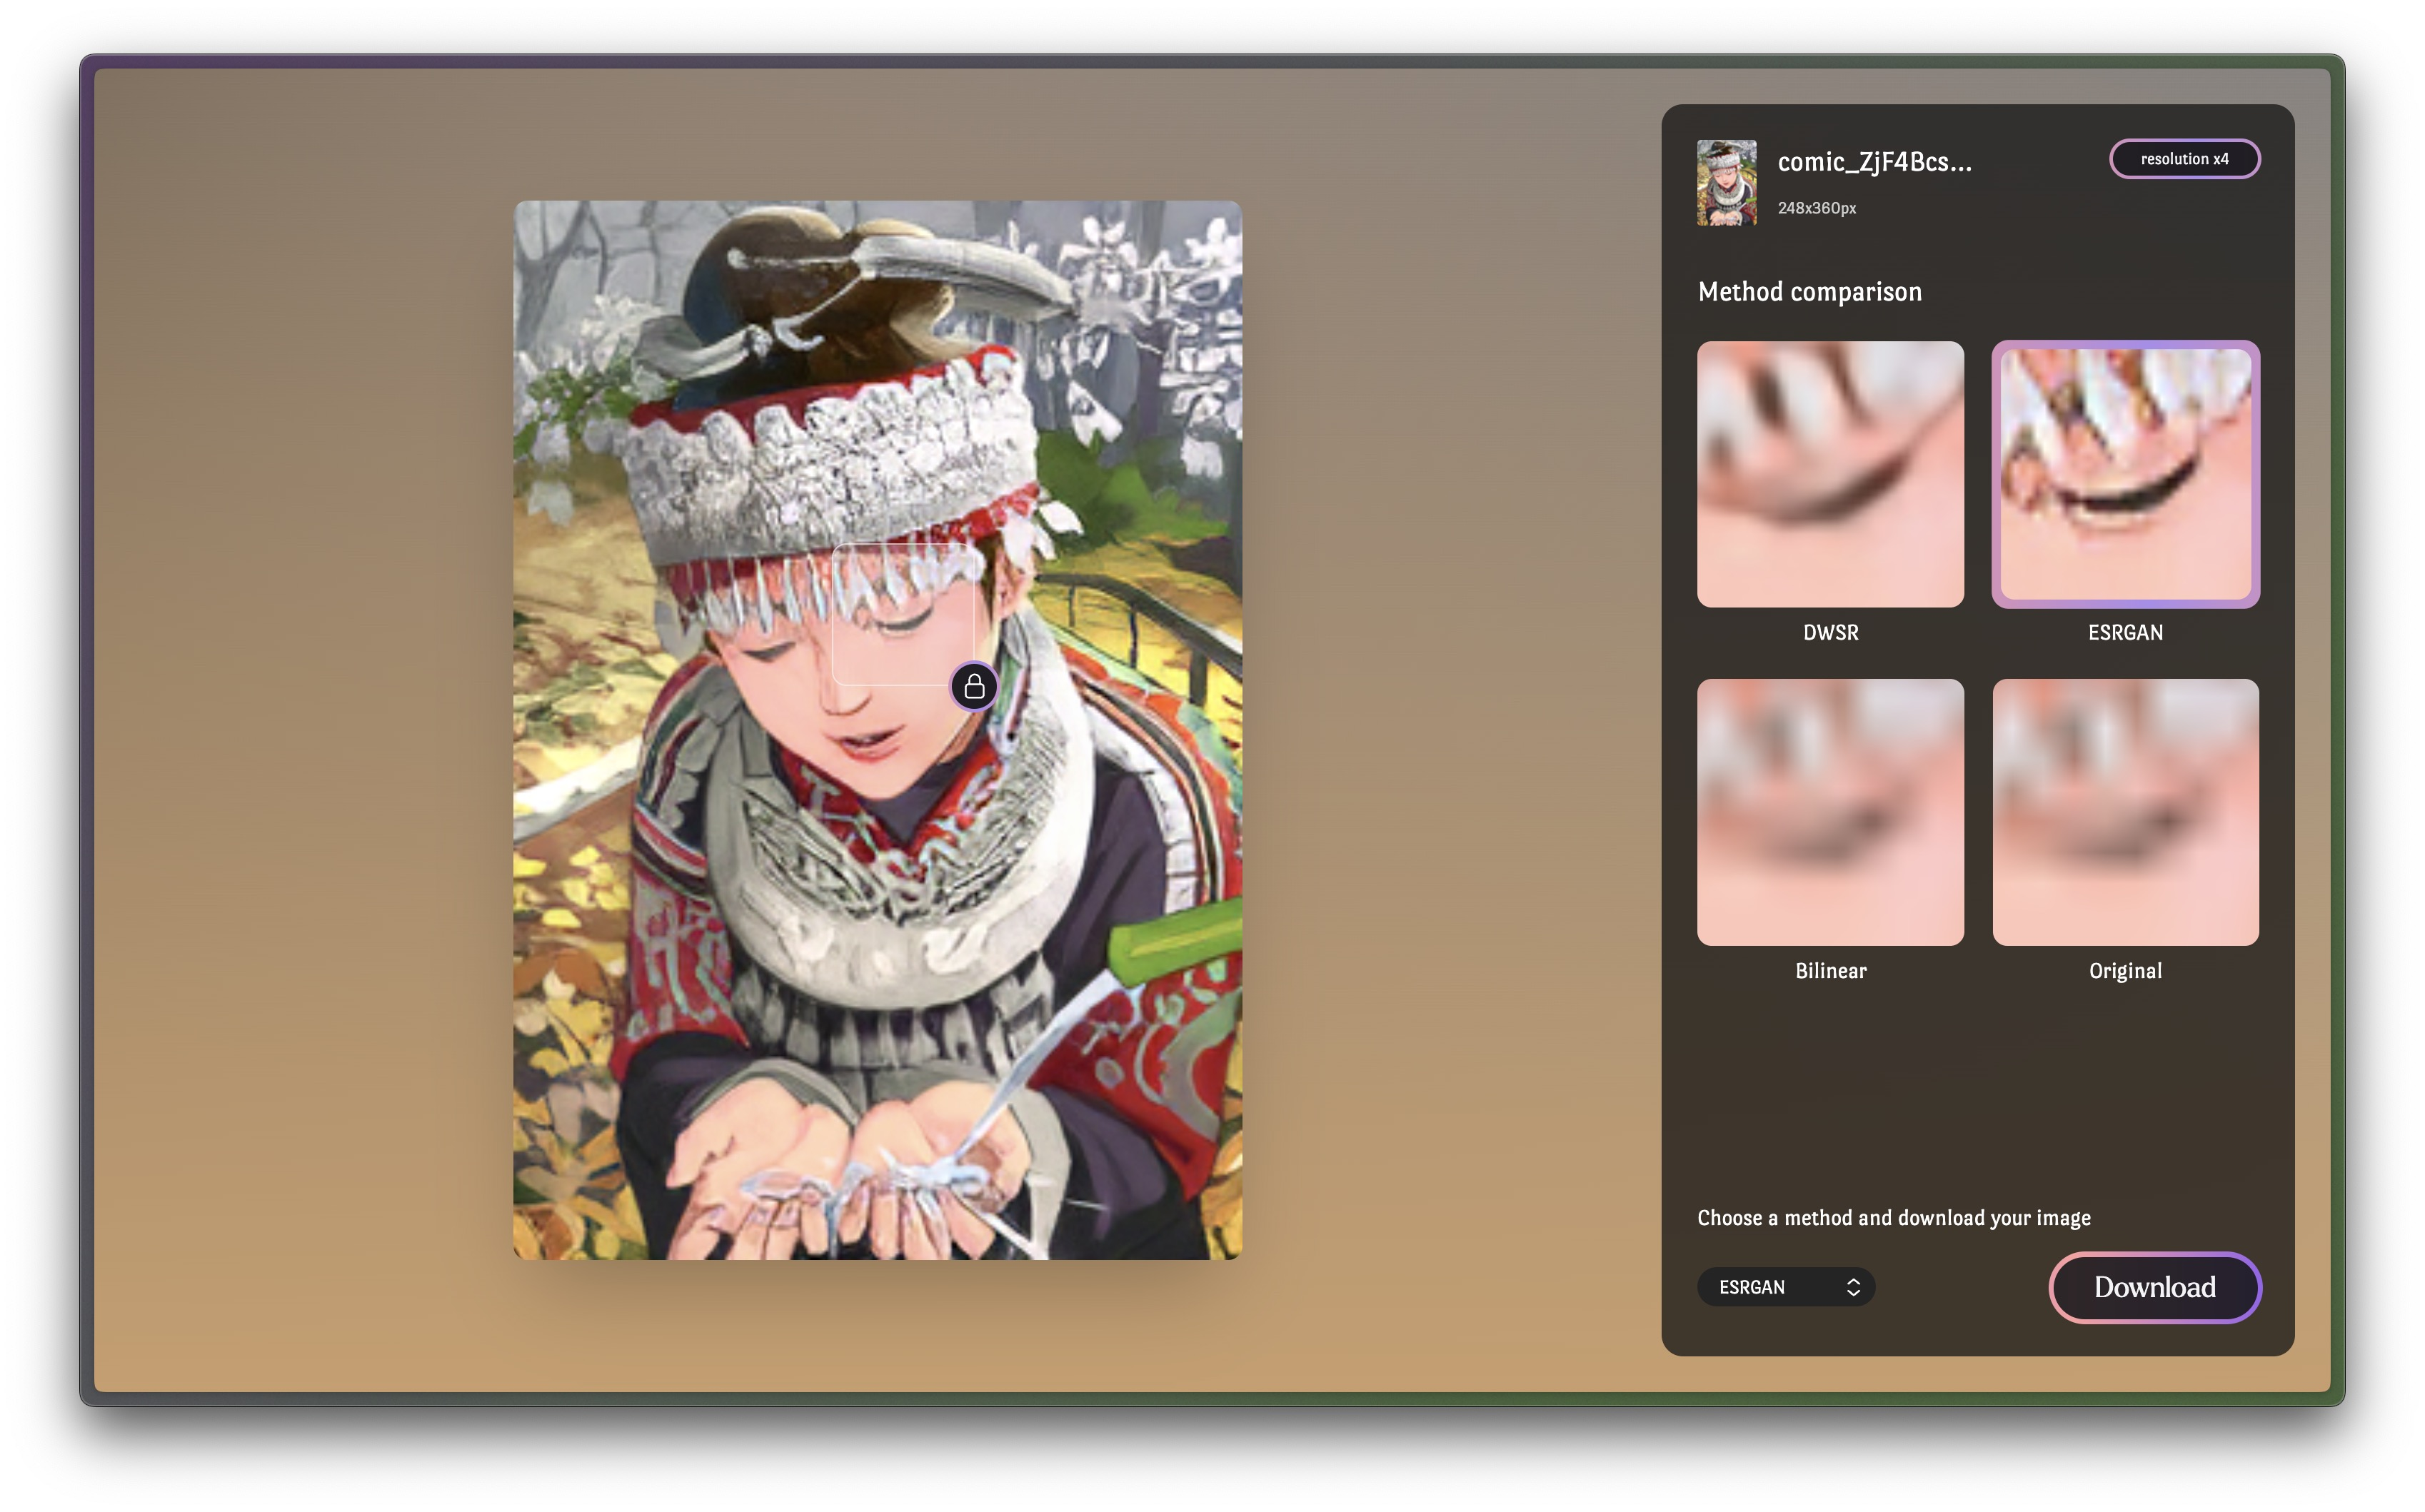
\includegraphics[width=0.9\linewidth]{Rozdziały/05.Porownanie_algorytmow/Obrazy/Zrzut ekranu comic.jpg}  
    \caption{Obraz \textit{comic.png} z zestawu testowego Set14 \cite{zeyde2010single}}
    \label{fig:image104}
\end{figure}

Ostatnim przykładem będzie rysunek techniczny z obrazu \ref{fig:image105}. Algorytm \textbf{ESRGAN} jest bardzo wrażliwy na kompresję jpg, w wyniku czego obraz wygląda nieprzyjemnie a czcionki są zbyt ostre.  Algorytm \textbf{DWSR} poradził sobie dużo lepiej z rekonstrukcją obrazu, czcionki są wyraźne i czytelne, a obraz nie jest mocno zniekształcony.

\begin{figure}[H]
    \centering
    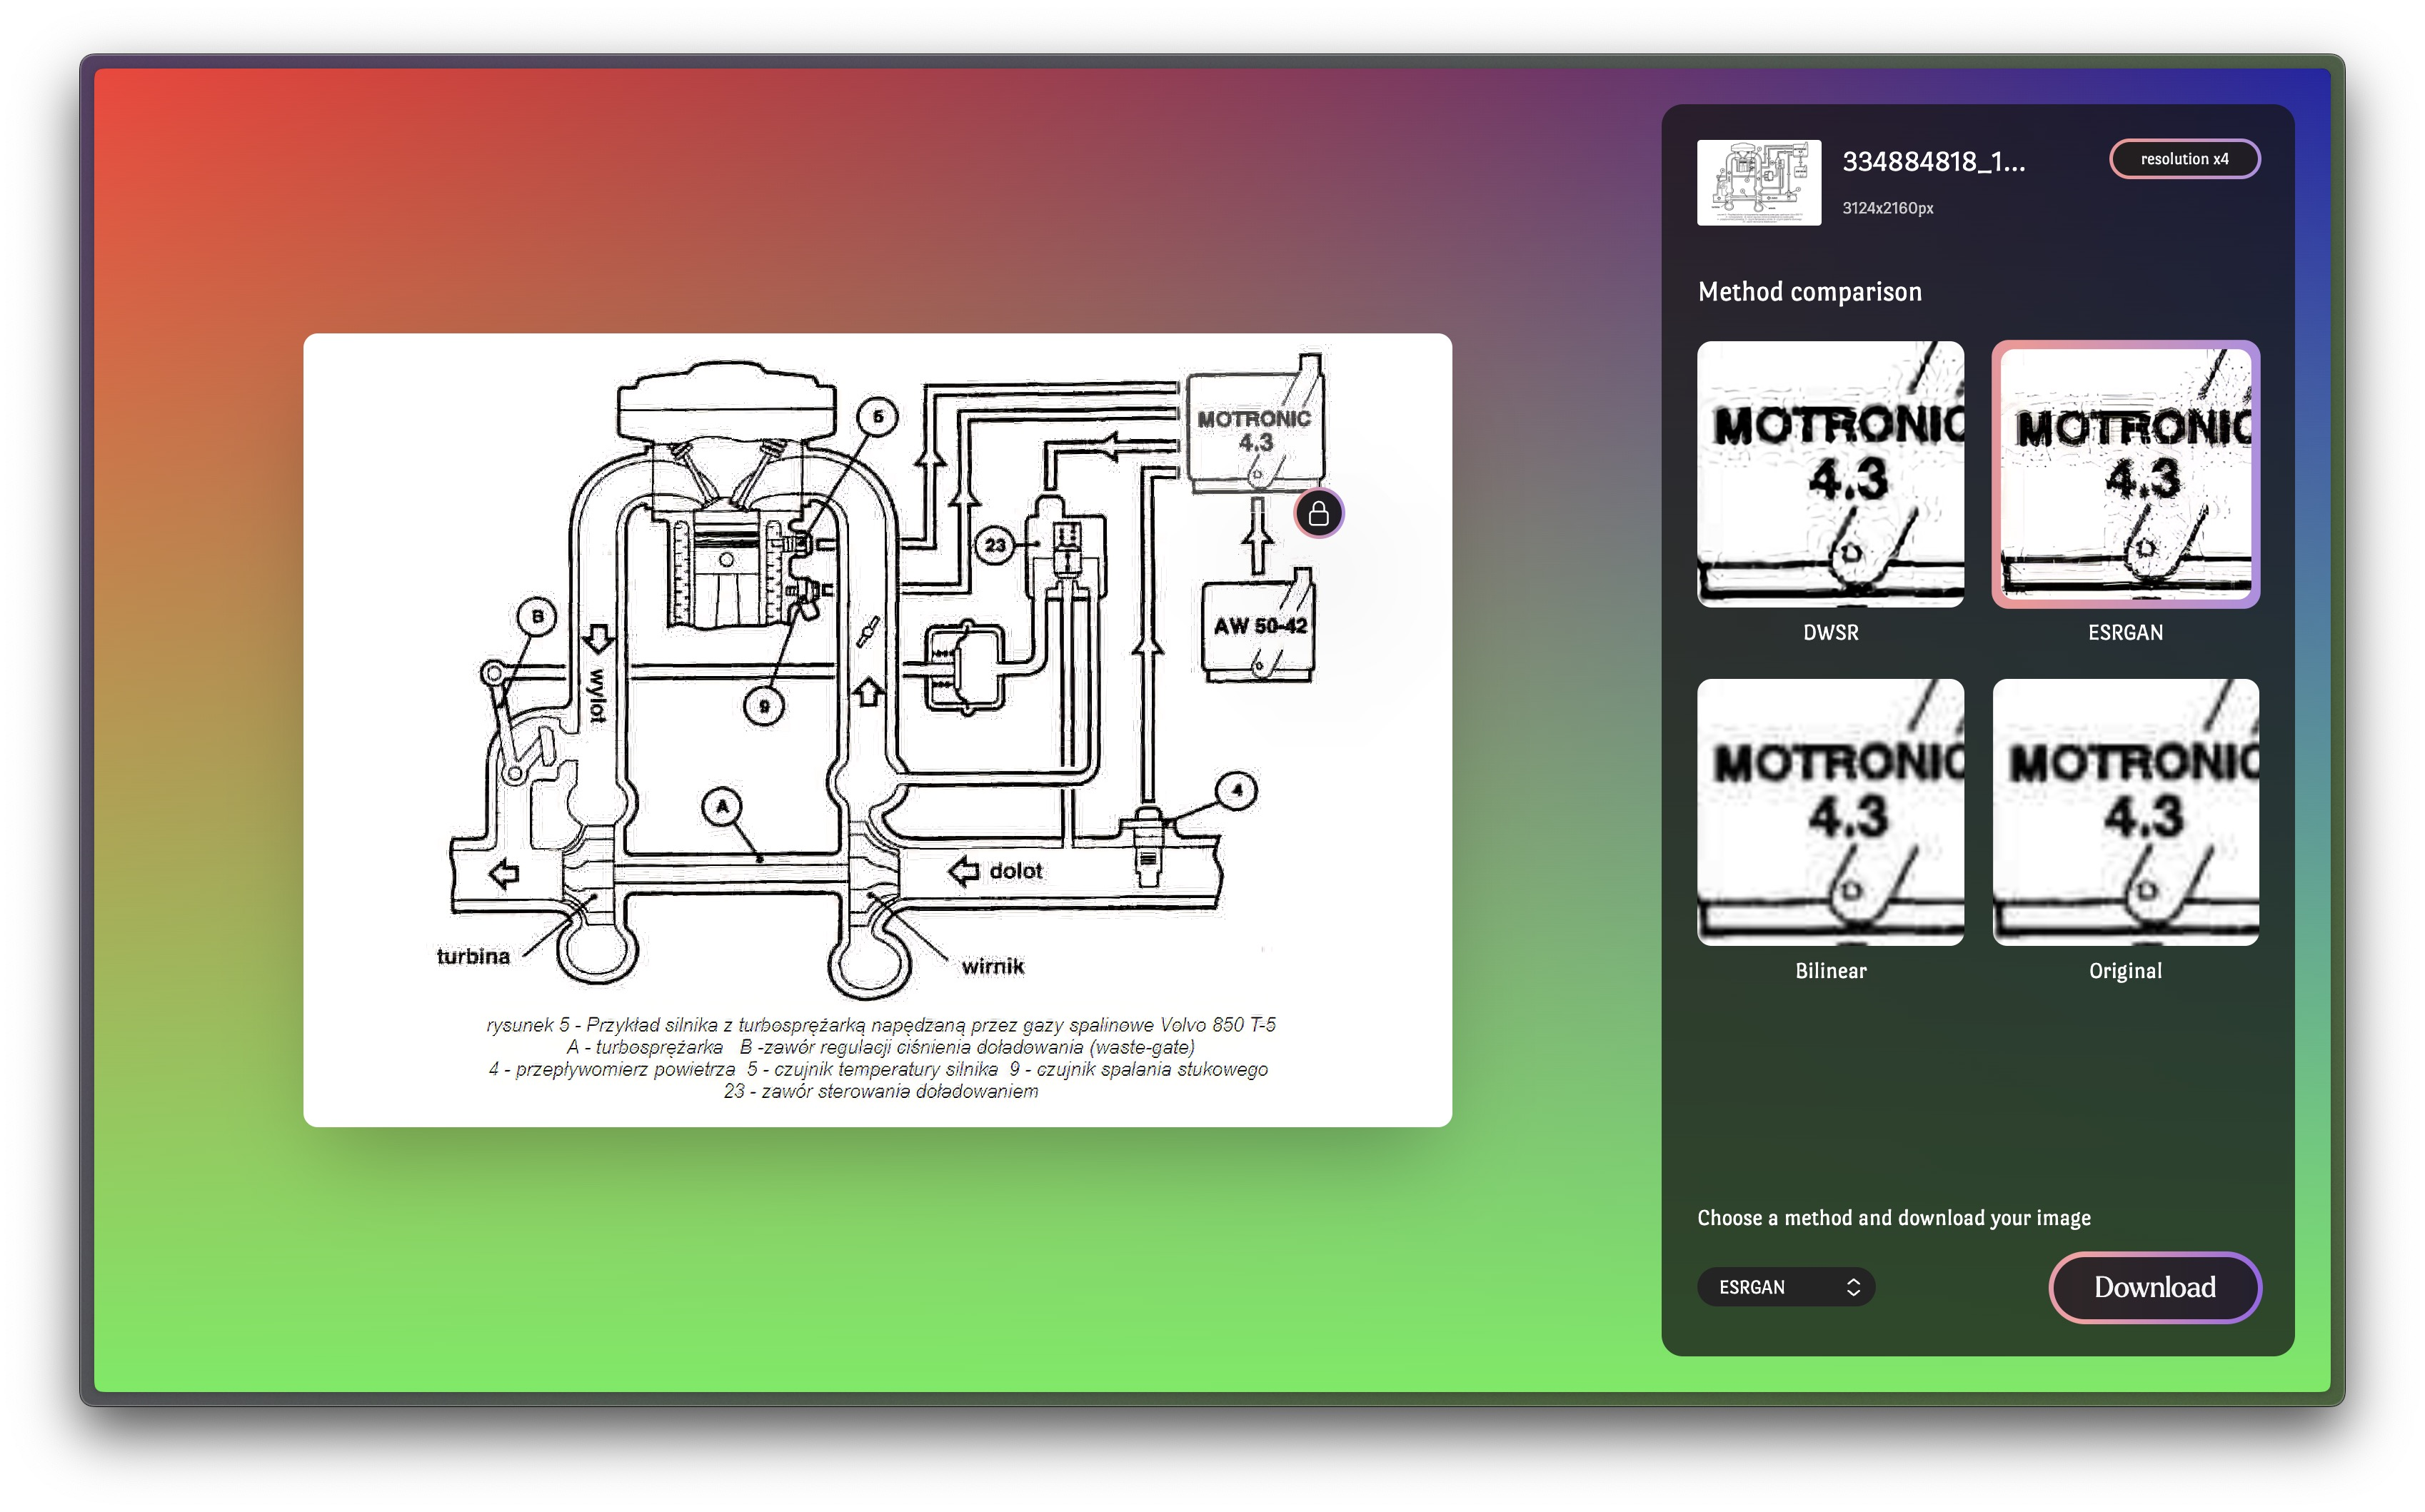
\includegraphics[width=0.85\linewidth]{Rozdziały/05.Porownanie_algorytmow/Obrazy/Zrzut ekranu 2023-12-12 o 14.20.22.jpg}  
    \caption{Schemat techniczny silnika z turbosprężarką ze strony \cite{zssplus} }
    \label{fig:image105}
\end{figure}

\section{Analiza wydajności}

Na podstawie rozdziałów traktujących o strukturach algorytmów \textbf{DWSR} i \textbf{ESRGAN} można zauważyć, że algorytm \textbf{ESRGAN} jest dużo bardziej skomplikowany. W związku z tym można przypuszczać, że algorytm \textbf{DWSR} będzie działał szybciej. W tym rozdziale sprawdzę jak wygląda wydajność obu algorytmów.

Do testów wydajności wykorzystałem obrazy z zestawu testowego \cite{guo2017deep} oraz \cite{zeyde2010single}. Testy zostały przeprowadzone na komputerze z procesorem \textbf{Intel Core i7-9750H} z systemem \textbf{MacOS}, więc niestety nie mogłem wykorzystać GPU do przyspieszenia obliczeń, ponieważ biblioteka \textbf{PyTorch} nie wspiera kart graficznych \textbf{AMD}, w którą wyposażony jest sprzęt.

\begin{figure}[H]
    \centering
    \begin{tikzpicture}
        \begin{axis}[
            xlabel={Rozdzielczość oryginalna (piksele)},
            ylabel={Czas (sekundy)},
            legend style={at={(rel axis cs:0,1)},anchor=north west}, % Zmienione położenie legendy
            ymajorgrids=true,
            grid style=dashed,
            width=0.95\textwidth, % Szerokość wykresu dopasowana do szerokości tekstu
            height=8cm, % Ustaw wysokość jeśli to potrzebne
        ]
        \addplot table [x=resolution, y=bilinear_time, col sep=comma] {Rozdziały/05.Porownanie_algorytmow/Obrazy/image_data.csv};
        \addlegendentry{Bilinear}
        \addplot table [x=resolution, y=dwsr_time, col sep=comma] {Rozdziały/05.Porownanie_algorytmow/Obrazy/image_data.csv};
        \addlegendentry{DWSR}
        \addplot table [x=resolution, y=esrgan_time, col sep=comma] {Rozdziały/05.Porownanie_algorytmow/Obrazy/image_data.csv};
        \addlegendentry{ESRGAN}
        \end{axis}
    \end{tikzpicture}

    \caption{Wykres czasu przetwarzania obrazów w zależności od rozdzielczości oryginalnej}
    \label{fig:time_chart}
\end{figure}
    


\section{Ograniczenia i wyzwania}


Dyskusja na temat ograniczeń obu metod i potencjalnych wyzwań w ich stosowaniu.